\documentclass[]{beamer}

\mode<presentation>
{
  \usetheme{Madrid}      % or try Darmstadt, Madrid, Warsaw, ...
  \usecolortheme{crane} % or try albatross, beaver, crane, ...
  \usefonttheme{default}  % or try serif, structurebold, ...
  \setbeamertemplate{navigation symbols}{}
  \setbeamertemplate{caption}[numbered]
  \setbeamercovered{transparent}
  \usefonttheme{serif}
} 

\usepackage[english]{babel}
\usepackage[utf8x]{inputenc}
\usepackage{mathtools, xcolor, soul, amsfonts, appendixnumberbeamer}
\graphicspath{ {images/} }


\title[]{Fraud detection using data mining techniques}
\author[]{Dariush Hasanpoor\, Mohsen Khaleghi}
\institute[]{Isfahan University Of Technology}
\date[]{Jun 23 2015}
\newcommand{\Xtri}{$\blacktriangleright$ }
\newcommand{\Ytri}{$\triangleright$ }
\newcommand{\itemXtri}{\item[\Xtri]}
\newcommand{\itemYtri}{\item[\Ytri]}
\renewcommand{\|}[1][.3em]{\hspace{#1}|\hspace{#1}}
\renewcommand{\,}[1][.3em]{,\hspace{#1}}
\newcommand\Wider[2][3em]{
\makebox[\linewidth][c]{
  \begin{minipage}{\dimexpr\textwidth+#1\relax}
  \raggedright#2
  \end{minipage}
  }
}
\newcommand*{\Scale}[2][4]{\scalebox{#1}{$#2$}}

\definecolor{light-blue}{HTML}{66AFE9}
\definecolor{light-red}{HTML}{F77B7B}
\definecolor{light-green}{HTML}{87D13E}

\begin{document}

\begin{frame}
  \titlepage
\end{frame}

\begin{frame}{Features}
\begin{figure}
\centering
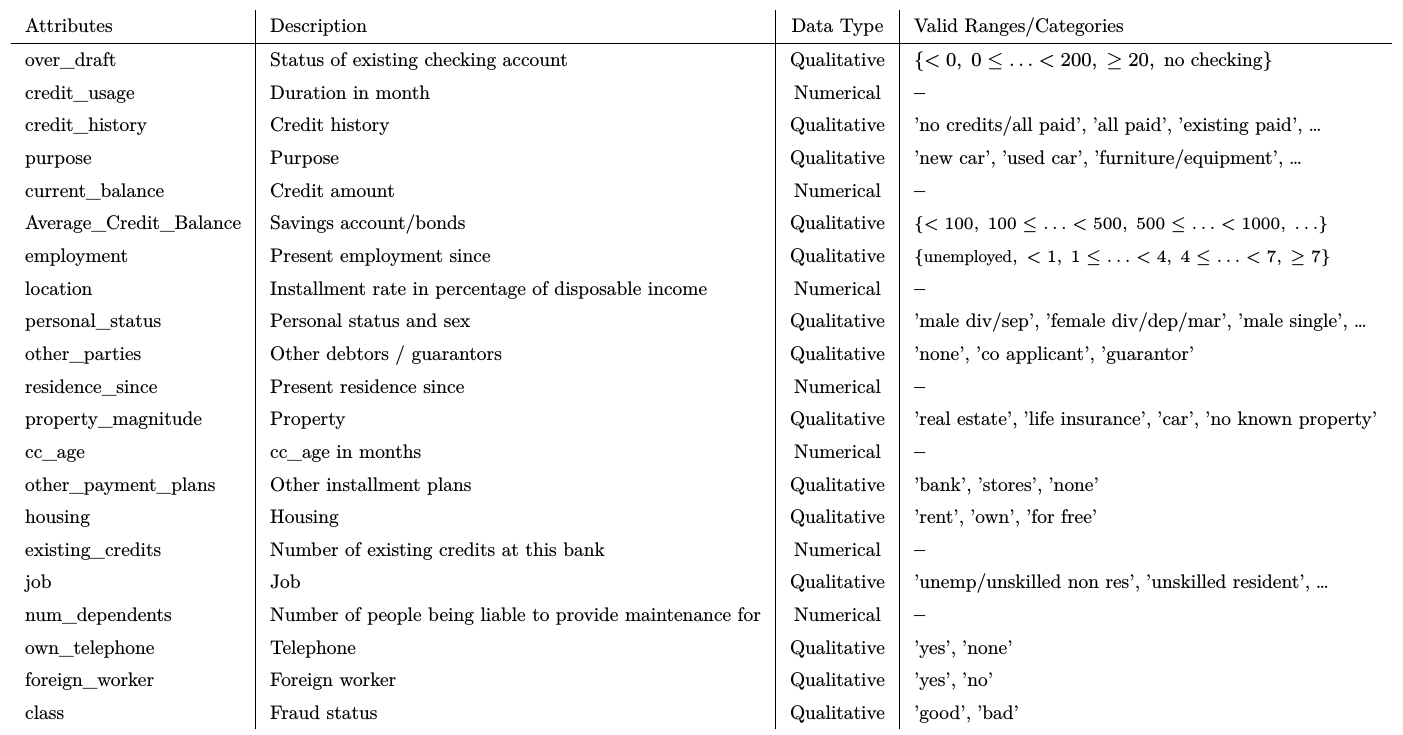
\includegraphics[width=\textwidth]{features}
\end{figure}
\end{frame}

\begin{frame}{Class distribution over predictors}
\begin{figure}
\centering
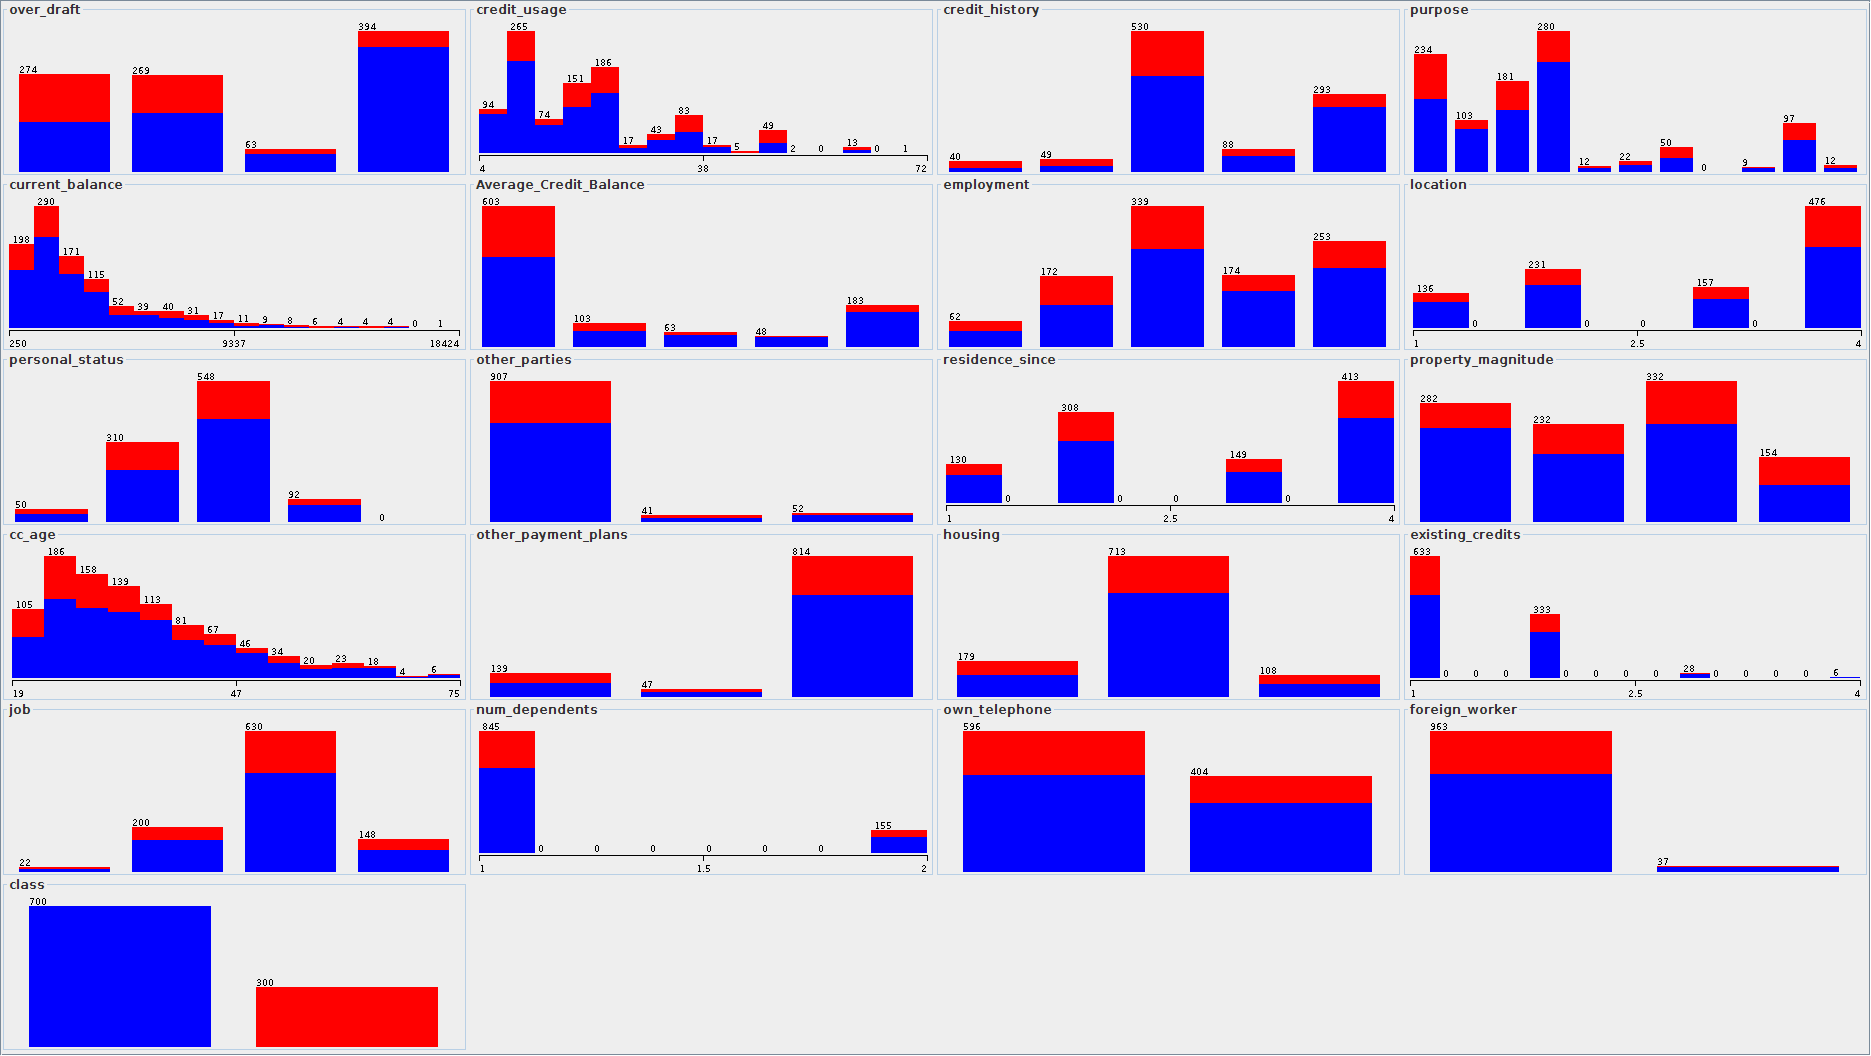
\includegraphics[width=\textwidth]{overall_dist}
\end{figure}
\end{frame}

\begin{frame}{Association Rules}
\begin{figure}
\centering
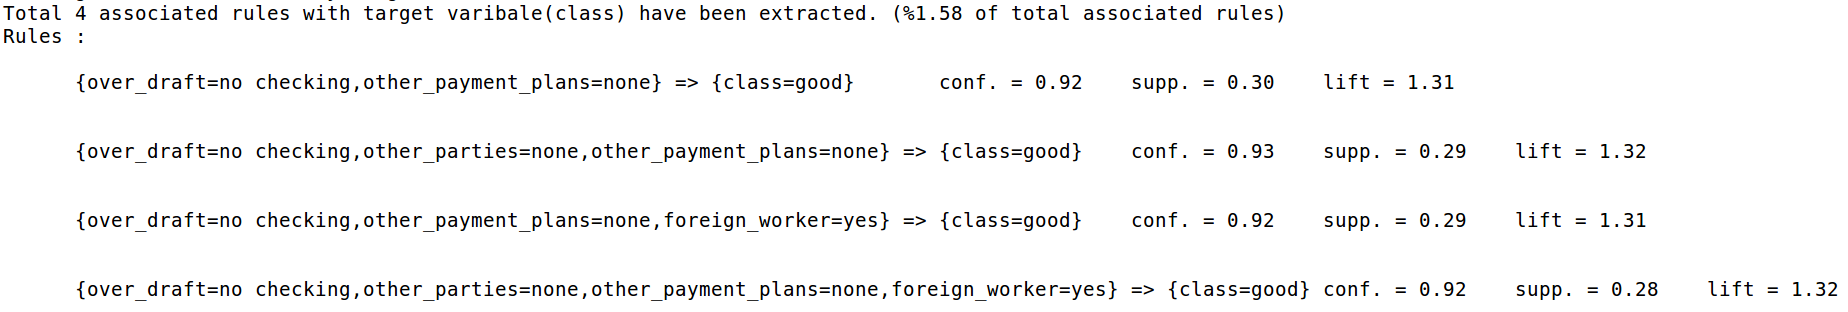
\includegraphics[width=\textwidth]{assoc}
\end{figure}
\end{frame}

\begin{frame}{Classifications}
\begin{table}[ht]\small
\centering
\def\arraystretch{1.5}
\begin{tabular}{l|c|c|c}
Measures & Naive Bayesian & SVM(kernel $\rightarrow$ rbfdot) & Decision Tree\\\hline
Accuracy & 0.76 & 0.77 & 0.72\\
95\% CI & (0.70, 0.80) & (0.71, 0.81) & (0.66, 0.77)\\
Sensitivity & 0.53 & 0.36 & 0.45\\
Specificity & 0.85 & 0.94 & 0.84\\
P-Value & 0.013 & 0.003 & 0.173
\end{tabular}
\end{table}
\end{frame}

\begin{frame}{Choquet Integral}
    \begin{itemize}
    \itemXtri Choquet Integral
    \item[]
        \begin{align*}
        &\mathcal{C}_\mu(x) = \sum_{i = 1}^n (x_{\tau(i)} - x_{\tau(i - 1)})\mu(\{\tau(i),\ldots,\tau(n)\})\\
        &\Scale[0.8]{x_{\tau(1)}{\leq}x_{\tau(2)}\leq\ldots{\leq}x_{\tau(n)}}\,\Scale[0.8]{x_{\tau(0)} = 0}
        \end{align*}
    \end{itemize}
    \pause
    \begin{align*}
    &\mu(\{\emptyset\}) = 0\,\mu(\{\text{NB}\,\text{SVM}\,\text{TR}\}) = 1\\
    &\mu(\{\text{NB}\}) = \mu(\{\text{SVM}\}) = \mu(\{\text{TR}\}) = {1 \over 3}\\
    &\mu(\{\text{NB}\,\text{SVM}\}) = 0.8\\
    &\mu(\{\text{NB}\,\text{TR}\}) = \mu(\{\text{SVM}\,\text{TR}\}) = {2 \over 3}
    \end{align*}
\end{frame}

\begin{frame}{Classifications Cont.}{With Choquet Integral}
\Wider{\begin{table}[ht]\scriptsize
\centering
\def\arraystretch{1.5}
\begin{tabular}{l|c|c|c|c}
Measures & Naive Bayesian & SVM(kernel $\rightarrow$ rbfdot) & Decision Tree & \textbf{FCI}\\\hline
Accuracy & 0.76 & 0.77 & 0.72 & \textbf{0.78}\\
95\% CI & (0.70, 0.80) & (0.71, 0.81) & (0.66, 0.77) & \textbf{(0.73, 0.83)}\\
Sensitivity & 0.53 & 0.36 & 0.45 & \textbf{0.52}\\
Specificity & 0.85 & 0.94 & 0.84 & \textbf{0.90}\\
P-Value & 0.013 & 0.003 & 0.173 & \textbf{0.0003}
\end{tabular}
\end{table}}
\end{frame}

\begin{frame}
\begin{center}
\Huge Thank You!
\end{center}
\end{frame}

\appendix
\begin{frame}{Classifications Cont.}{Decision Tree}
\Wider{\begin{figure}
\centering
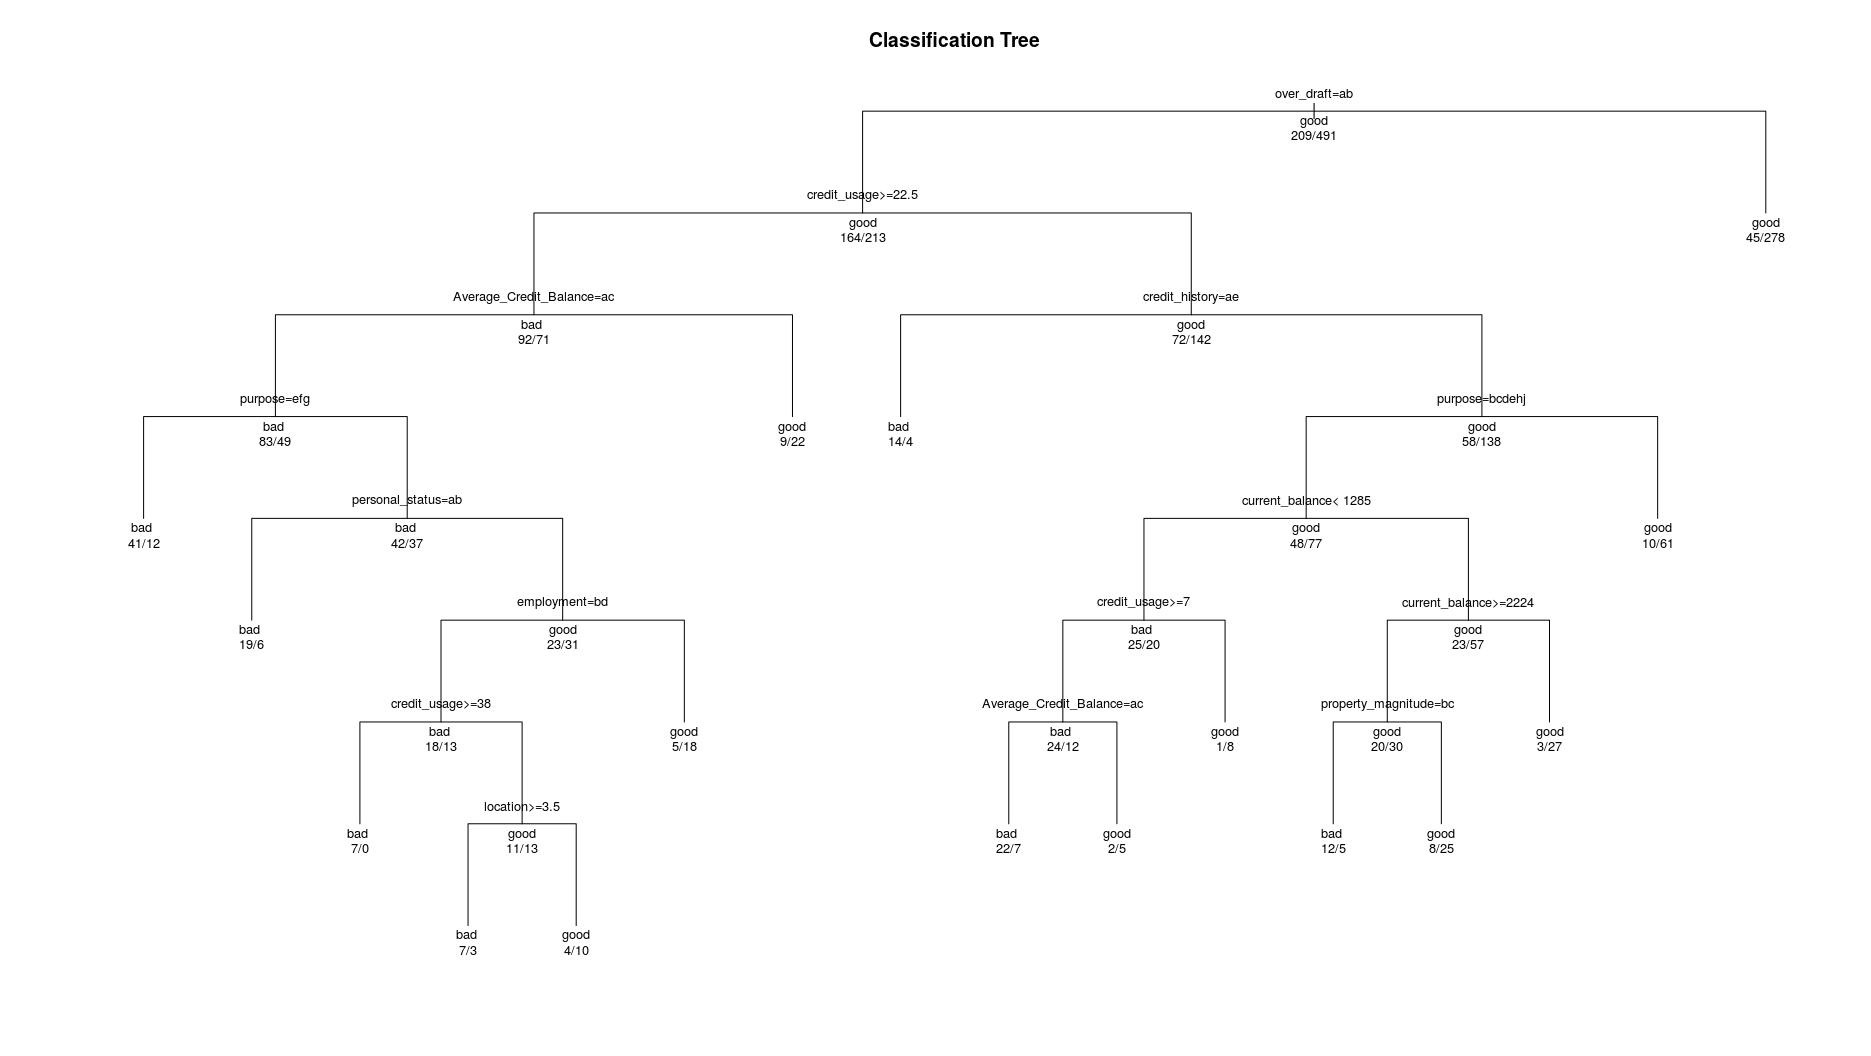
\includegraphics[width=\textwidth]{dt}
\end{figure}}
\end{frame}


\end{document}